\documentclass[11pt, oneside]{article}   	% use "amsart" instead of "article" for AMSLaTeX format


% \usepackage{draftwatermark}
% \SetWatermarkText{Draft}
% \SetWatermarkScale{5}
% \SetWatermarkLightness {0.9} 
% \SetWatermarkColor[rgb]{0.7,0,0}

%
%	TikZ
%
\usepackage{tikz}
\usetikzlibrary{angles, quotes}
\usetikzlibrary{calc}
\usetikzlibrary{intersections}
\usetikzlibrary{arrows,backgrounds,calc,patterns,angles,quotes,shapes,calc,decorations,through,hobby,lindenmayersystems,matrix}
\usepackage{tikz-cd}
\tikzset{>=latex}                                                      % default to LaTeX arrow head
\usepackage{tkz-euclide}
\usepackage{pgfplots}
\tikzset{>=latex}                                                       % default to LaTeX arrow head
% Set the default arrow head style to be LaTeX (TikZ)
\tikzcdset{every arrow/.append style={-latex}}
%
%
%
\usepackage{geometry}                   % See geometry.pdf to learn the layout options
\geometry{letterpaper}                  % ... or a4paper or a5paper or ... 
%\geometry{landscape}                   % Activate for for rotated page geometry
%\usepackage[parfill]{parskip}          % Activate to begin paragraphs with an empty line rather than an indent
\usepackage{graphicx}                   % Use pdf, png, jpg, or eps with pdflatex; use eps in DVI mode
\usepackage{amssymb}
\usepackage{mathrsfs}
\usepackage{hyperref}
\usepackage{url}
\usepackage{subcaption}
\usepackage{authblk}
\usepackage{amsmath}
\usepackage{commath}                                                    % get \norm{x}
\usepackage{mathtools}
\usepackage{graphicx}
\usepackage[export]{adjustbox}
\usepackage{hyperref}
\usepackage{alltt}
\usepackage{color}
\usepackage[utf8]{inputenc}
\usepackage[english]{babel}
\usepackage{float}
\usepackage{bigints}
\usepackage{braket}
\usepackage{siunitx}
\usepackage{relsize}
\usepackage{braket}
\usepackage{amsthm}

\usepackage{lmodern}
\usepackage[T1]{fontenc}

\usepackage{halloweenmath}
\usepackage{blochsphere}


%
% compatability
%
\pgfplotsset{compat=1.17} 

\usepackage{tikz-3dplot}

%
%	get the x and y coordinates out of a coordinate
%
\makeatletter
\newcommand{\gettikzxy}[3]{%
  \tikz@scan@one@point\pgfutil@firstofone#1\relax
  \edef#2{\the\pgf@x}%
  \edef#3{\the\pgf@y}%
}
\makeatother



\begin{document}

\begin{equation*}
\tau_d := \{A \mid \text {$A$ is open in $X$} \} = \{A \subseteq X \mid \text{forall $x$ in $A$ there exists an $\epsilon$ such that $B_{\epsilon}(x) \subseteq A$}\}
\end{equation*}

\vspace{5.0em}
\bigskip
\bigskip

\begin{tikzcd}[row    sep={35pt},
               column sep={40pt}]
     & X \arrow[d,dashed, "\exists! \tau"] \arrow[ddl,swap,"\sigma_{1}"] \arrow[ddr,"\sigma_{2}"] \\
     & V \times W \arrow[dl,"\rho_{1}"] \arrow[dr,swap,"\rho_{2}"]                                \\
   V & & W 
\end{tikzcd}


\vspace{5em}

\noindent
$A,B,S \in \mathcal{C}$ and $f: A \to B$


\bigskip
\begin{math}
- \times S =
\begin{cases} 
    A \times S  \hspace{10em} \mathrel{\#} A \in \mathcal{C} \\ 
    f \times \text{id}_{S}: A \times S \to B \times S \hspace{1.55em} \mathrel{\#} (a,s) \mapsto (f(a),s)
\end{cases}
\end{math}

\bigskip
\bigskip
%
%	Use shift left and shift right to separate the 
%	two arrows between A and B
%
\begin{tikzcd}[column sep={30pt}]
A \arrow[r,"f_{1}",shift left] \arrow[r,"f_{2}",swap,shift right] & B \arrow[r,"g"] & C
\end{tikzcd}

\bigskip
\noindent
For sets a mapping $g:B \to C$ is said to be \emph{injective}
if for $b_{1}, b_{2} \in B$ we have $g(b_{1}) = g(b_{2}) \Rightarrow b_{1} = b_{2}$.

\bigskip
\noindent
Not a good definition because it looks inside the objects. Rather, in category
theory we define a more general concept, \emph{monomorphism}. A morphism $g:B \to C$
is said to be a monomorphism if for all $f_{i}: A \to B$ we have $gf_{1} 
= gf_{2} \Rightarrow f_{1} = f_{2}$.



\vspace{3.0em}


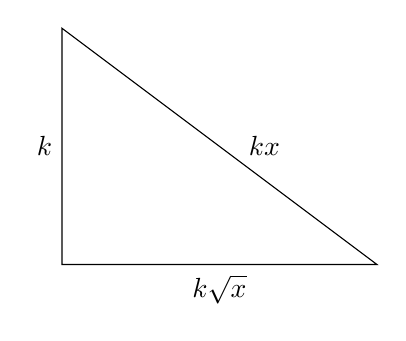
\begin{tikzpicture}
    % Define named points for the vertices of the right triangle
    \coordinate (A) at (0,0);
    \coordinate (B) at (4,0);
    \coordinate (C) at (0,3);
    
    % Draw the right triangle using the named points
    \draw (A) -- (B) -- (C) -- cycle;
    
    \draw [draw=none] (A) -- (B) node [midway,below,yshift=-0.1mm] {$k\sqrt{x}$};
    \draw [draw=none] (A) -- (C) node [midway,left] {$k$};
    \draw [draw=none] (B) -- (C) node [midway,right, xshift=0.25cm] {$kx$};


    
    % Label the vertices
%    \node[below left] at (A) {A};
%    \node[below right] at (B) {B};
%    \node[above left] at (C) {C};
\end{tikzpicture}


\begin{center}
  \begin{tikzcd}
     A \arrow[loop above, distance=1cm, in=120, out=60]{} 
       \arrow[loop left, distance=1cm, in=150, out=210]{} 
       \arrow[loop below, distance=1cm, in=240, out=300]{}
       \arrow[loop right, distance=1cm, in=30, out=330]{} 
  \end{tikzcd}
\end{center}

%
%	Draw the function composition triangle
%
\begin{center}
   \begin{tikzcd} [column sep={50pt},
                   row    sep={40pt}]
        A \arrow[r,"f"] \arrow[d, swap, "g \circ f",] & B \arrow[ld,"g"] \\
        C 
   \end{tikzcd}
\end{center}

\vspace{0.75cm}

%
%	Draw the picture
%
%
%          		 F(f)
%		   F(A) ------> F(B)
%	  		|            |
%	  η_{A} |            |  η_{B}
%	        v            v
%	       G(A) ------> G(B)
%                G(f)
%
%
\begin{center}
\begin{tikzcd} [column sep={75pt},
                row    sep={50pt}]
    F(A) \arrow[r, "F(f)"] \arrow[d, swap, "\eta_{A}"] & F(B) \arrow[d, "\eta_{B}"] \\
    G(A) \arrow[r, swap, "G(f)"]                       & G(B)
\end{tikzcd}
\end{center}


%
%	Set a few parameters
%
\def \scale {0.85}                                                                      % scale arrow labels
%
%
%
\medskip
%
%	Draw the picture
%
%
%          		 F(f)
%		   F(A) ------> F(B)
%	  		|            |
%	  η_{A} |            |  η_{B}
%	        v            v
%	       G(A) ------> G(B)
%                G(f)
%
%
\begin{center}                                                                          % center the tikzpicture
   \begin{tikzpicture}
      \matrix[matrix of math nodes,                                                     % use a TikZ matrix for the vertices
              column sep={100pt,between origins},
              row    sep={60pt,between origins}] (m)
              {                                                                         % matrix looks like:
                |[name=FA]|F(A) & |[name=FB]|F(B) \\                                    % F(A) F(B)
                |[name=GA]|G(A) & |[name=GB]|G(B) \\                                    % G(A) G(B)
              }; 
              \draw[->] (FA) edge node [midway,above,scale=\scale] {$F(f)$} (FB)        % F(A) -> F(B) by F(f)
                        (GA) edge node [midway,below,scale=\scale] {$G(f)$} (GB)        % G(A) -> G(B) by G(f)
                        (FA) edge node [midway,left,scale=\scale]  {$\eta_{A}$} (GA)    % F(A) -> G(A) by \eta_{A}
                        (FB) edge node [midway,right,scale=\scale] {$\eta_{B}$} (GB);   % F(B) -> G(B) by \eta_{B}
   \end{tikzpicture}
\end{center}





%	
%	\usepackage{halloweenmath}
%
%
%	Set space and frame thickness
%
\setlength {\fboxsep} {0.50em}					% get more space between fcolorbox and content
\setlength {\fboxrule}{0.80pt}					% set the outside fcolorbox line thickness
%												%
%												%
%												%
\begin{figure}[H]								% build the figure
  \centering									% center everything
  \resizebox{1.00 \textwidth}{!} {				% resize the figure if you like
    \fcolorbox{black}{white} {					% make the outside frame black
      \setlength {\fboxrule}{0.60pt}			% set the inside fcolorbox line thickness
      \fcolorbox{orange}{white}{				% make the inside frame orange					
        \begin{math}							% math mode
          G (\mathbat) \!						% do some halloween math (minus some space)						
          \xrightswishingghost{n = \langle \bigskull,\mathghost \rangle} \!
          {\boldsymbol {\color{orange}\bigpumpkin}}_{i = 1}^{n} 
          H_{i}(\mathwitch*) 					% 
        \end{math}								% exit math mode
      }											% end fcolorbox{orange}{white}
    }											% end fcolorbox{black}{white} 
  }												% end resizebox
  \caption{Happy Halloween!}					% caption the figure
  \label{figure:happy_halloween}				% get a label if needed
\end{figure}									% done


\vspace{3em}


\begin{figure}[H]
  \centering
  \fcolorbox{black}{white}{
    \resizebox{0.750 \textwidth}{!} {
      \begin{math}
         A \xrightwitchonbroom*[abc\dots z]{f_{1}+\dots+f_{n}} B
           \xrightwitchonbroom*{f_{1}+\dots+f_{n}} C
           \xrightwitchonbroom*[abc\dots z]{} D
      \end{math}
     }
  }
  \caption{Happy Halloween!}
\end{figure}

\vspace{3.0mm}

\begin{math}
  \mathwitch
  \bigpumpkin
  \bigskull
  \mathcloud
  \rightbroom
  \mathghost
  \mathbat
\end{math}

\bigskip
%
%
%

\begin{figure}[H]
  \centering
  \resizebox{0.50 \textwidth}{!} {                      % resize figure here if you want
    \begin{tikzpicture}[scale=0.60]                     % can also scale the tikzpicture here
       \coordinate (O)          at (0,0);               % origin
       \coordinate (Xstart)     at (-1,0);              % x-axis 
       \coordinate (Xend)       at (10,0);              % x-axis
       \coordinate (Ystart)     at (0,-1);              % y-axis
       \coordinate (Yend)       at (0,8);               % y-axis
       \coordinate (EP)         at (8,5);               % endpoint (U)
       
	   \gettikzxy{(EP)}{\slopex}{\slopey}
%
%
%
%      \newcommand{\slope} {5/8};                       % the U line goes through the origin so y = mx = \slope*x
       
               
       \def \slope {\fpeval{\slopey/\slopex}};			% the U line goes through the origin so y = mx = \slope*x

%
%
%
\node [] at (10,10) {\slope};
%
%
%
       \coordinate (SP)         at (-2,\slope*-2);      % start point (U)
       \coordinate (uEP)        at (2,\slope*2);        % end point (u)
       \coordinate (vEP)        at (3,\slope*3);        % end point (v)
       \coordinate (u+vEP)      at (5,\slope*5);        % end point (u+vEP)
%	
%	draw axes and linear subspace U
%
       \draw[thin,->,black] (Xstart) -- (Xend) node[right] {$x$};       % x axis
       \draw[thin,->,black] (Ystart) -- (Yend) node[above] {$y$};       % y axis
       \draw[thick,magenta] (SP) -- (EP) node [right,xshift=1.50mm,yshift=1.50mm] 
                        {$\color{black} U \subset \mathbb{R}^{2}$}; 
%
%	draw vectors u, v and u+v
%    
		\draw[thick,green,->](O) -- (uEP) node
                     [right,below,xshift=2.00mm,yshift=0.50mm] 
                     {$\color{green}\mathbf{u}$}; 
		\draw[thick,red,->](uEP) -- (vEP) node
                     [right,xshift=0.25mm,yshift=-1.0mm]
                     {${\color{red}\mathbf{v}}
                       {\color{black}=} 
                       {\color{black} \lambda}
                       {\color{green}\mathbf{u}}$};  
		\draw[thick,blue,->](vEP) -- (u+vEP) node
                     [right,xshift=0.25mm,yshift=-1.25mm]  
                     {${\color{blue}\mathbf{w}}
                       {\color{black}=}
                       {\color{green}\mathbf{u}}
                       {\color{black} +}
                       {\color{red}\mathbf{v}}$}; 
   \end{tikzpicture}
 }
\caption{The line $U$ is a linear subspace of $\mathbb{R}^{2}$}
\label{fig:linear_subspace}
\end{figure}




%
% bloch sphere
%
\bigskip
\begin{figure}[H]
\centering
  \resizebox{0.50 \textwidth}{!} {	
  
  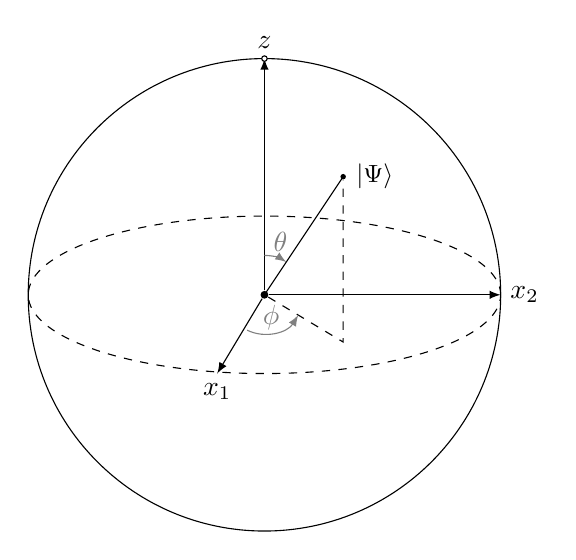
\begin{tikzpicture}

  % Define radius
  \def\r{3}

  % Bloch vector
  \draw (0, 0) node[circle, fill, inner sep=1] (orig) {} -- (\r/3, \r/2) node[circle, fill, inner sep=0.7, label=right:{\small ${\ket{\Psi}}$}] (a) {};
  \draw[dashed] (orig) -- (\r/3, -\r/5) node (phi) {} -- (a);

  % Sphere
  \draw (orig) circle (\r);
  \draw[dashed] (orig) ellipse (\r{} and \r/3);

  % Axes
  \draw[->] (orig) -- ++(-\r/5, -\r/3) node[below] (x1) {$x_1$};
  \draw[->] (orig) -- ++(\r, 0) node[right] (x2) {$x_2$};
  \draw[->] (orig) -- ++(0, \r) node[above] (x3) {$z$};
  \draw[fill=white] (0,\r) circle (0.035);   									% draw center of circle




  % Angles
  \pic [draw=gray, text=gray, ->, "$\phi$"] {angle = x1--orig--phi};
  \pic [draw=gray, text=gray, <-, "$\theta$", angle eccentricity=1.4] {angle = a--orig--x3};

\end{tikzpicture}
     
  }																					 								% end resizebox                                                            
 \caption{The Bloch Sphere}
% \label{fig:bloch_sphere}
\end{figure}

\bigskip
\bigskip
			
%
%
%
\begin{figure}[H]
  \centering
  \resizebox{0.50 \textwidth}{!} {                              % resize figure if you want
  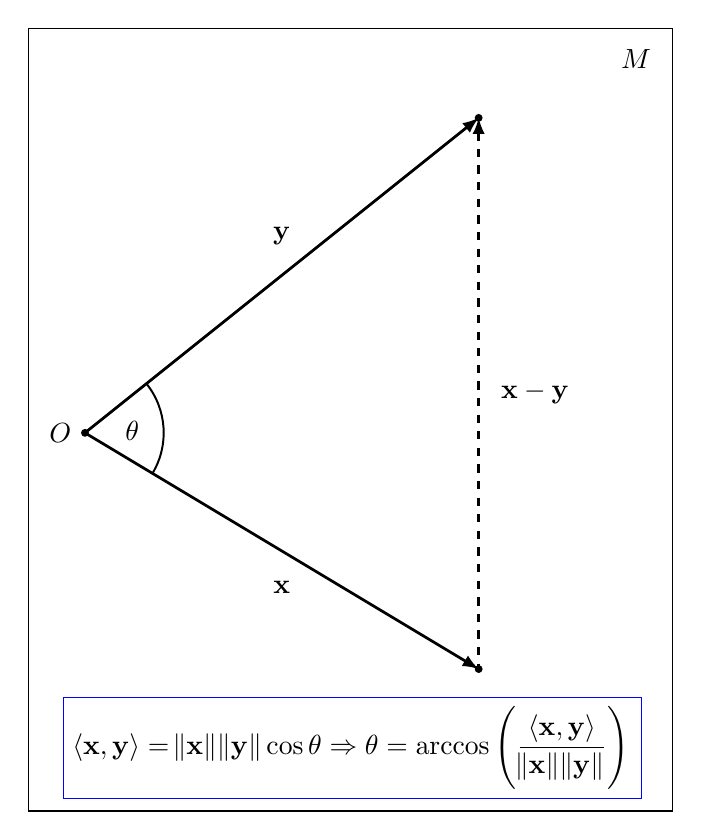
\begin{tikzpicture} [scale=1,framed]							% add a tikz frame
       \coordinate (O)                  at (0,0);               % origin O
       \coordinate (Box)                at (0,-4);				% put the box here (roughtly)
       \coordinate (Xstart)             at (-1,0);              % x-axis 
       \coordinate (Xend)               at (10,0);              % x-axis
       \coordinate (Ystart)             at (0,-1);              % y-axis
       \coordinate (Yend)               at (0, 7.5);            % y-axis
       \coordinate (T)					at (5,4);				% Top point
       \coordinate (B)					at (5,-3);				% bottom point
       \coordinate (TM)					at (2.5,2.00);			% (x,y_1) coordinate
       \coordinate (BM)					at (2.5,-1.50);			% (x,y_2) coordinate 
       \coordinate (M) 					at (7,4.75);			% draw M in upper right corner (x and y generate a plane M)    
%
%
%	Don't draw coordinate system
%       
%	\draw[ultra thick,-latex](Xstart) -- (Xend) node[right,scale=1.75] {$x$};				% x axis
%	\draw[ultra thick,-latex](Ystart) -- (Yend) node[above,scale=1.75] {$y$};				% y axis
%
%
		\draw [line width=0.35mm,-latex] (O) -- (T) node [midway,above,yshift=0.25cm]  {$\mathbf{y}$};	% draw y (top vector)
		\draw [line width=0.35mm,-latex] (O) -- (B) node [midway,below,yshift=-0.25cm] {$\mathbf{x}$};	% draw x (bottom vector)
		\draw [line width=0.35mm,dashed,latex-] (T) -- (B) node [midway,right,xshift=0.15cm]			% draw x-y
			{$\mathbf{x} - \mathbf{y}$};																% continue drawing x - y
		\fill [black] (T) circle (0.05);																% draw a dot, top of x - y
		\fill [black] (B) circle (0.05);																% draw a dot, bottom of x - y
		\node[] at (M) {$M$};

%
%	Draw the angle, box, etc
%       
		\pic [draw,line width=0.25mm,angle radius=10mm,angle eccentricity=1.2]				% or \pic [...,"${...}$"] {angle = ...}; 
			{angle = BM--O--TM};															% this draws the angle
		\fill [black] (O) circle (0.05) node[below,left,xshift=-0.05cm] {$O$};				% label the origin
		\node [yshift=0.25mm,xshift=6.0mm] at (O) {$\theta$};								% label theta 		
		\node[xshift=7.075cm,below,left,draw,rectangle,color=blue,thin,scale=1] at (Box)	% get \theta = ... in the right place
			{$\color{black}{\langle \mathbf{x},\mathbf{y} \rangle = 
			\norm{\mathbf{x}}\norm{\mathbf{y}} \cos \theta \Rightarrow 
			\theta = \arccos \Bigg(\dfrac{\langle \mathbf{x},\mathbf{y} \rangle}
			{\norm{\mathbf{x}} \norm{\mathbf{y}}} \Bigg )}\hspace{0.10em}$};
%
%	done
%       
   \end{tikzpicture}
  }  																						% end \resizebox
 \caption{Geometric interpretation of $\langle \mathbf{x},\mathbf{y} \rangle$}
 \label{fig:geometric_dot_product}
\end{figure}
%
%
%
\bigskip
%
%
%
\begin{figure}[H]
\centering
  \resizebox{0.60 \textwidth}{!} {                              % resize figure if you want
  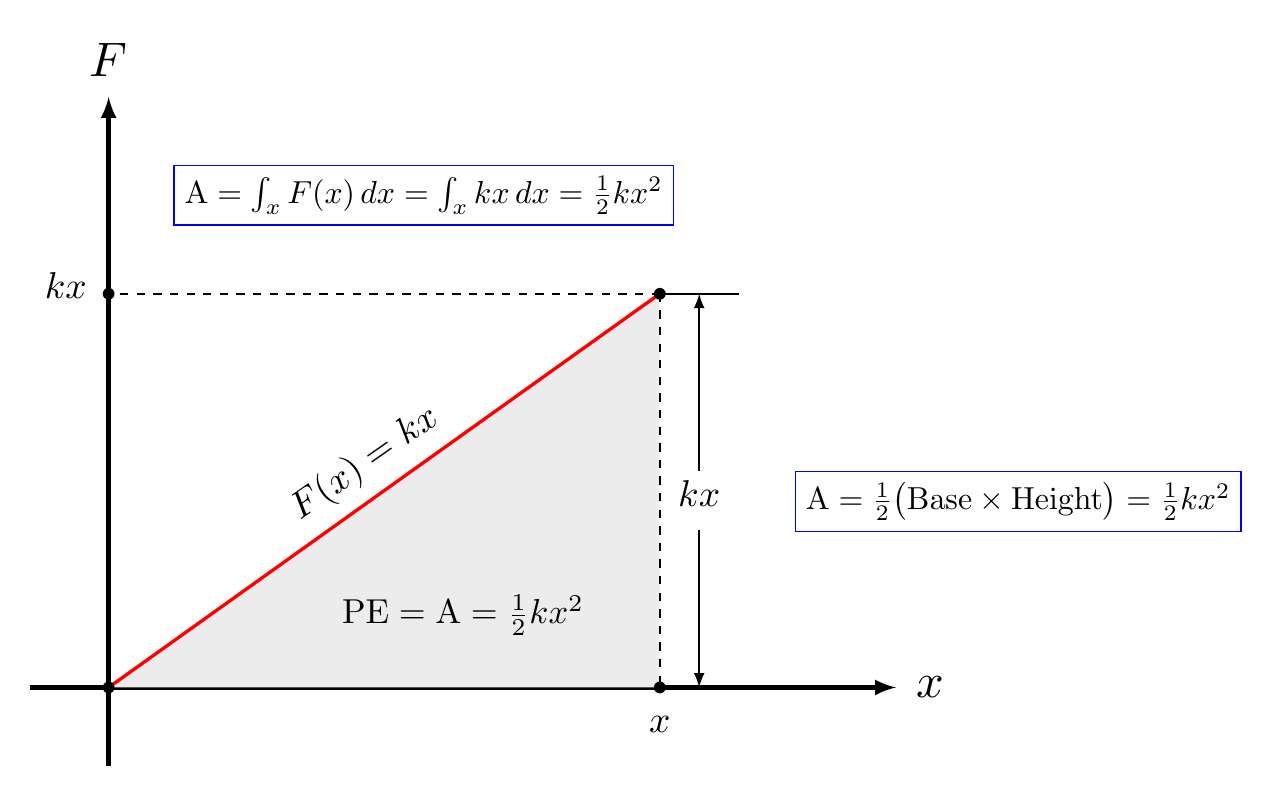
\begin{tikzpicture}
       \coordinate (O)                  at (0,0);               % origin O
       \coordinate (Xstart)             at (-1,0);              % x-axis 
       \coordinate (Xend)               at (10,0);              % x-axis
       \coordinate (Ystart)             at (0,-1);              % y-axis
       \coordinate (Yend)               at (0, 7.5);            % y-axis
       \coordinate (EP)                 at (7,5);               % endpoint of the F vs. x line
       \coordinate (EPO)                at (8,5);               % endpoint origin
       \coordinate (TopHalf1)           at (7.5,2.75);          % top half of kx line
       \coordinate (TopHalf2)           at (7.5,5);             % top half of kx line
       \coordinate (BottomHalf1)        at (7.5,2);             % bottom half of kx line
       \coordinate (BottomHalf2)        at (7.5,0);             % bottom halft of kx line
       \coordinate (X)                  at (7,0);               % x coordinate of kx line
       \coordinate (Y)					at (0,5);
       \coordinate (A)					at (4.0,6.25);			% A = ... rectangle
%
%
%
       
       \draw[ultra thick,-latex](Xstart) -- (Xend) node[right,scale=1.75] {$x$};      % x axis
       \draw[ultra thick,-latex](Ystart) -- (Yend) node[above,scale=1.75] {$F$};      % y axis
       \draw [draw=none, fill=gray!15] (O) -- (EP) -- (X) -- cycle;
       \draw [draw=none] (O) -- (X) node[midway,above,scale=1.25,yshift=0.40cm,xshift=0.80cm] 
       				{${\text{PE} = \text{A} = \frac{1}{2}kx^2}$};
       \draw[very thick,red](O) -- (EP) node [left,above,midway,scale=1.35,rotate=35] 
       				{${\color{black}{F(x) = kx}}$}; 
       \draw[thick,dashed](EP) -- (X) coordinate []; 
       \fill [black] (O)  circle (0.075);
       \fill [black] (EP) circle (0.075);
       \fill [black] (X)  circle (0.075) node [below,yshift=-0.20cm,scale=1.35] {$x$};
       \draw [thick] (EP) -- (EPO) [];

%
%	Surely there is a better way to do this but this is what I came up with
%
       \draw [latex-, thick] (TopHalf2) -- (TopHalf1) node [below, yshift=0.05cm,scale=1.35] {$kx$};
       \draw [-latex, thick] (BottomHalf1) -- (BottomHalf2) [];
%
%	Show kx on the F axis
%
       \draw [thick,dashed] (EP) -- (Y) node [left,xshift=-0.10cm,yshift=0.10cm,scale=1.35] {$kx$};
       \fill [black] (Y) circle (0.075);
%
%	Draw the rectangle with A = ...
%
	   \node [draw,rectangle,blue,scale=1.15] at (A) 
	   		{$\color{black}{\text{A} = 
	   		  \int_{x} F(x) \, dx    =
			  \int_{x} kx \, dx      = 
			  \frac{1}{2}kx^{2}}$
			  };
%
%
%

	   \node [draw,rectangle,blue,scale=1.15] at (11.55,2.36) 
	   		{$\color{black}{\text{A} = \frac{1}{2} \big (
	   		  \text{Base} \times \text{Height} \big )  = \frac{1}{2} kx^{2}}$
			  };

       
 %       \fill [red] (8.6,2.40) circle (0.075);
    
%
%	done
%       
   \end{tikzpicture}
  }  % end \resizebox
 \caption{Potential Energy of a Simple Harmonic Oscillator}
 \label{fig:PE}
\end{figure}

\bigskip
\bigskip
%
%	draw the transformation: rectangle in the uv-plane
%
\begin{figure}[H]
\centering
  \resizebox{0.60 \textwidth}{!} {                      % resize figure if you want
  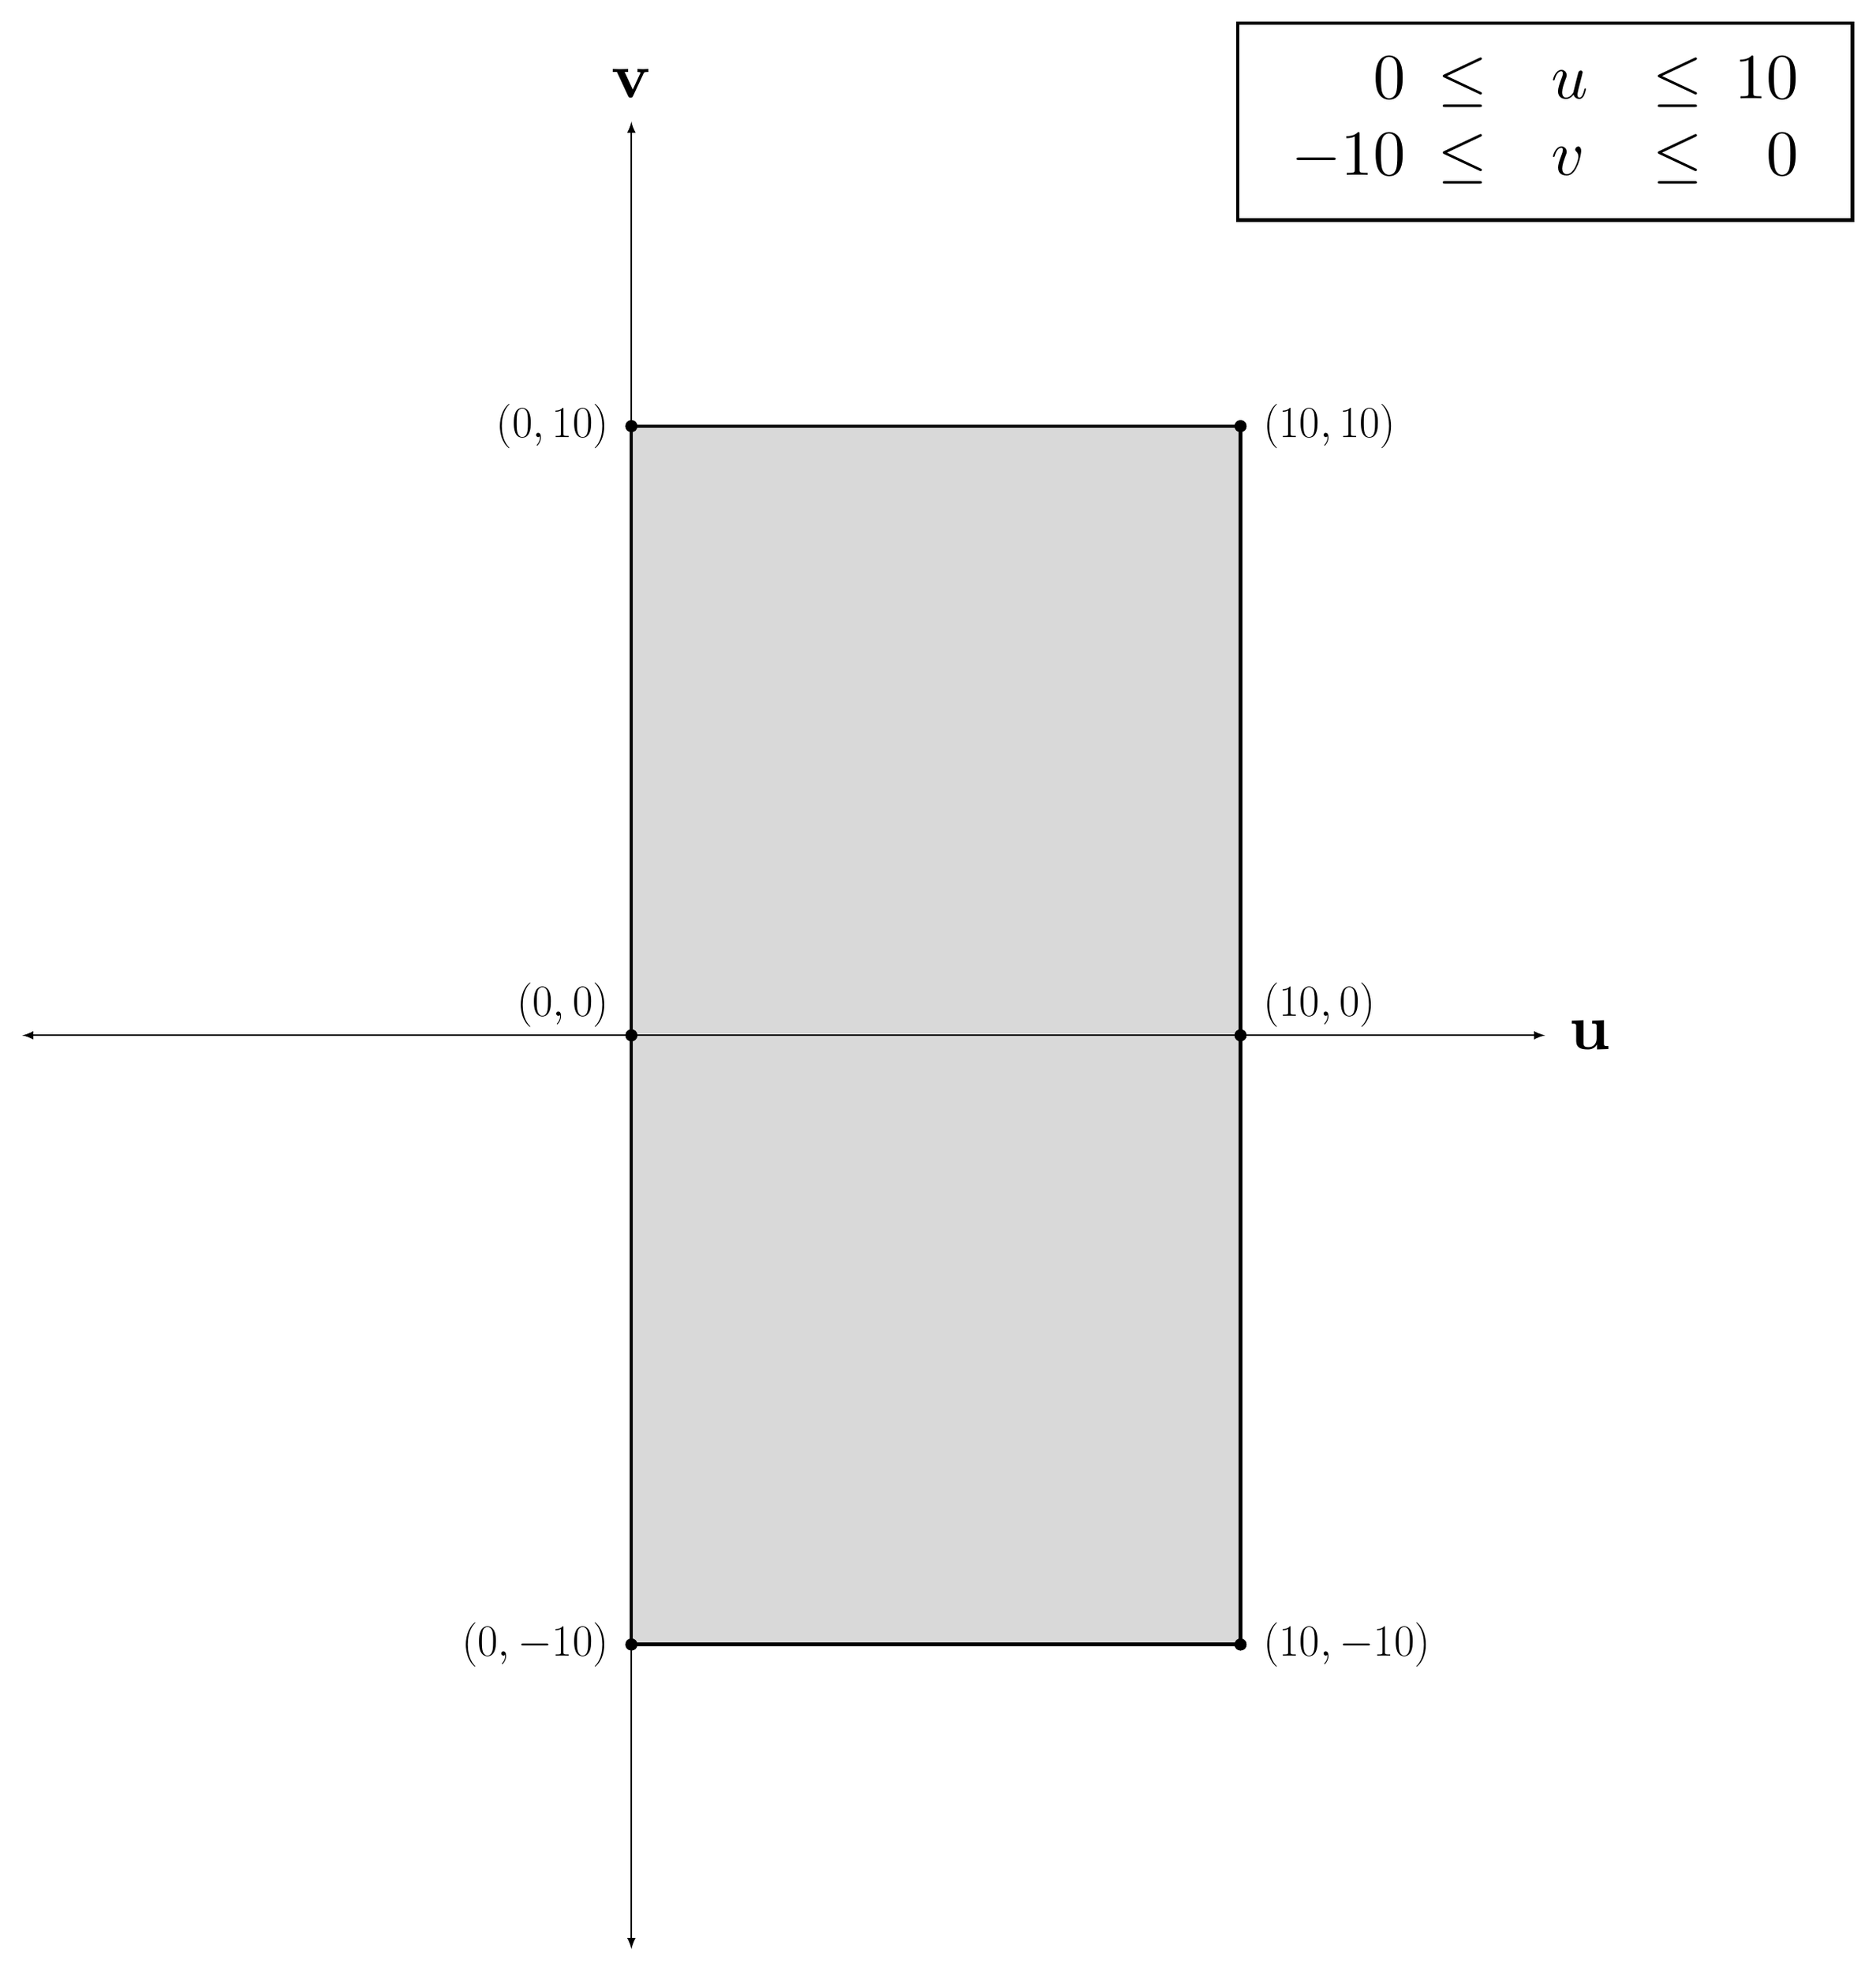
\begin{tikzpicture}
       \coordinate (O)          at (0,0);		% origin O
       \coordinate (Xstart)     at (-10,0);             % x-axis out to 8
       \coordinate (Xend)       at (15,0);              % x-axis out to 8
       \coordinate (Ystart)     at (0,-15);             % y-axis up to 6
       \coordinate (Yend)       at (0, 15);             % y-axis up to 6
       \coordinate (xy1)        at (0,-10);             % parallelogram point
       \coordinate (xy2)        at (0,10);              % parallelogram point
       \coordinate (xy3)        at (10,10);             % parallelogram point
       \coordinate (xy4)        at (10,-10);            % parallelogram point
       \coordinate (xy5)        at (10,0);				% parallelogram point

%
%	draw parallelogram
%
       \draw [ultra thick,fill=gray!30] (xy1) -- (xy2) -- (xy3) -- (xy4) -- cycle;
       \fill [black] (O)   circle (0.10) node[font=\huge,above,left,xshift=-0.25cm,yshift=0.5cm]  {$(0,0)$};
       \fill [black] (xy1) circle (0.10) node[font=\huge,left,xshift=-0.25cm]                     {$(0,-10)$};
       \fill [black] (xy2) circle (0.10) node[font=\huge,left,xshift=-0.25cm]                     {$(0,10)$};
       \fill [black] (xy3) circle (0.10) node[font=\huge,right,xshift=0.25cm]                     {$(10,10)$};
       \fill [black] (xy4) circle (0.10) node[font=\huge,right,xshift=0.25cm]                     {$(10,-10)$};
       \fill [black] (xy5) circle (0.10) node[font=\huge,above,right,xshift=0.25cm,yshift=0.50cm] {$(10,0)$};
%    r
%	draw axes making sure axes are on top
%
       \draw[thick,latex-latex](Xstart) -- (Xend) node[right,scale=3] {${\mathbf{u}}$};				% u axis
       \draw[thick,latex-latex](Ystart) -- (Yend) node[above,scale=3] {${\mathbf{v}}$};				% v axis
       
       
      \node[ultra thick,draw,rectangle,scale=3] at (15,15) {$\begin{array}{rrlrr}
                                                                0 \!\!\!  &\leq&  u &\leq& \!\!\! 10 \\
                                                               -10 \!\!\! &\leq&  v &\leq& 0
                                                             \end{array}$};
                                                                

      % \node[ultra thick,draw,rectangle,scale=3] at (15,15) {${0 \leq u \leq 10}$};
      % \node[ultra thick,draw,rectangle,scale=3] at (15,20) {${-10 \leq v \leq 0}$};


%
%	done
%       
   \end{tikzpicture}
  }																										% end \resizebox
 \caption{The transformed parallelogram is a rectangle in the $uv$-plane}
 \label{fig:uv_plane}
\end{figure}





%%%%

%
%	draw parallelogram for example
%
\begin{figure}[H]
\centering
  \resizebox{0.60 \textwidth}{!} {                      % resize figure if you want
  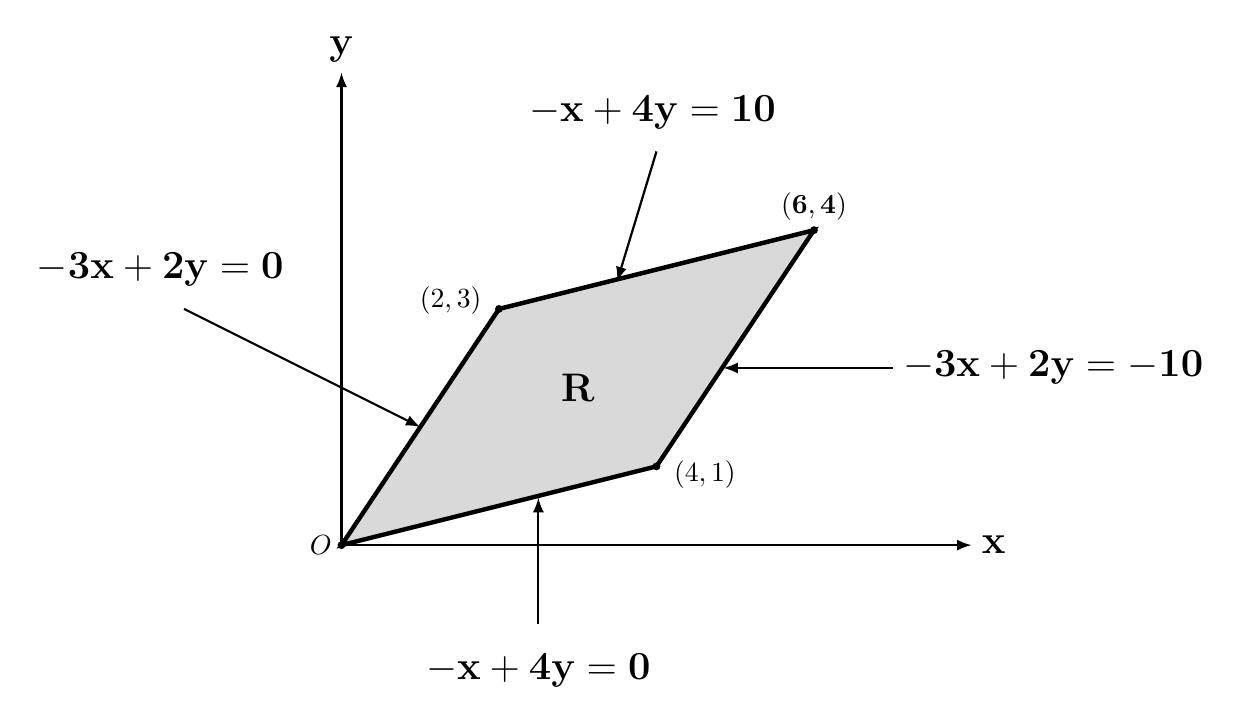
\begin{tikzpicture}
       \coordinate (O)          at (0,0);               % origin O
       \coordinate (Xend)       at (8,0);               % x-axis out to 8
       \coordinate (Yend)       at (0,6);               % y-axis up to 6
       \coordinate (C1)         at (2,3);               % parallelogram point
       \coordinate (C2)         at (6,4);               % parallelogram point
       \coordinate (C3)         at (4,1);               % parallelogram point
       \coordinate (C)          at (3,2);               % center of parallelogram is at C
%
%	coordinates for equations
%  
       \coordinate (D1)         at (1.00, 1.50);
       \coordinate (D2)         at (-2.00,3.00);
       \coordinate (E1)         at (3.50, 3.35);
       \coordinate (E2)         at (4.00, 5.00);
       \coordinate (F1)         at (4.85, 2.25);
       \coordinate (F2)         at (7.00, 2.25);
       \coordinate (G1)         at (2.50, 0.60);
       \coordinate (G2)         at (2.50,-1.00);
%
%	draw axes
%
     \draw[thick,-latex] (O) -- (Xend) coordinate [label={[right] {\Large ${\mathbf{x}}$}}];	% x axis
     \draw[thick,-latex] (O) -- (Yend) coordinate [label={[above] {\Large ${\mathbf{y}}$}}];	% y axis
%
%	draw parallelogram
%
     \draw [ultra thick,fill=gray!30]  (O) -- (C1) -- (C2) -- (C3) -- cycle;
     \node[color=black,font=\Large] at (C) {${\mathbf{R}}$};
     \fill [black] (O)  circle (0.05) node[below,left] {$O$};
     \fill [black] (C1) circle (0.05) node[yshift=1.0mm,xshift=-1.0mm,left] {$(2,3)$};
     \fill [black] (C2) circle (0.05) node[above] {${\mathbf{(6,4)}}$};
     \fill [black] (C3) circle (0.05) node[yshift=-1.00mm,xshift=1.0mm,right] {$(4,1)$};
%
%	draw equations of each size
%       
     \draw [thick,latex-] (D1) -- (D2) coordinate [label={[font=\Large,right,xshift=-2.0cm,yshift=0.50cm] 
                ${\mathbf {-3x + 2y = 0}}$}];
     \draw [thick,latex-] (E1) -- (E2) coordinate [label={[font=\Large,right,xshift=-1.75cm,yshift=0.5cm] 
                ${\mathbf {-x + 4y = 10}}$}];
     \draw [thick,latex-] (F1) -- (F2) coordinate [label={[font=\Large,right]
                ${\mathbf {-3x + 2y = -10}}$}];
     \draw [thick,latex-] (G1) -- (G2) coordinate [label={[font=\Large,below,yshift=-0.25cm] 
                ${\mathbf {-x + 4y = 0}}$}];
  \end{tikzpicture}
  }	
  \caption{Equations of the Sides of the Parallelogram}
  \label{fig:parallelogram_sides}
\end{figure}


%
%	draw parallelogram for example
%
\begin{figure}[H]
\centering
  \resizebox{0.40 \textwidth}{!} {                              % resize figure if you want
  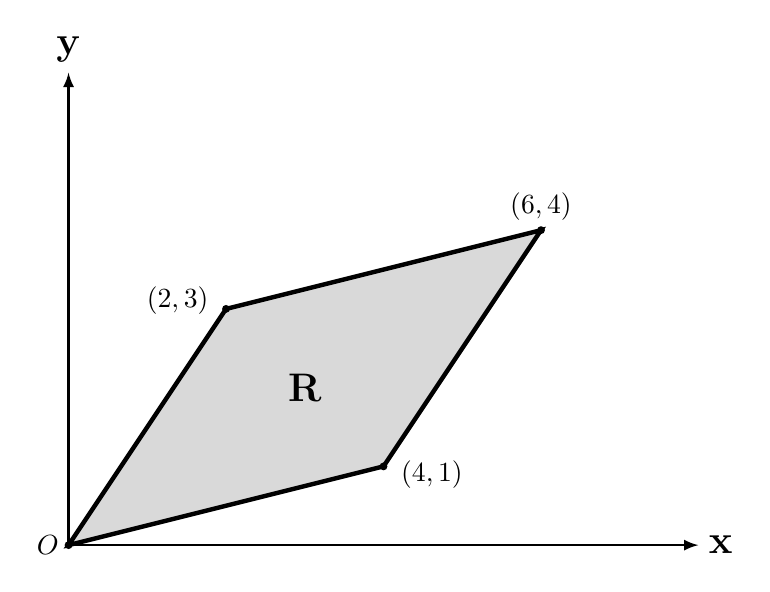
\begin{tikzpicture}
       \coordinate (O)          at (0,0);                       % origin O
       \coordinate(Xend)        at (8,0);                       % x-axis out to 8
       \coordinate(Yend)        at (0,6);                       % y-axis up to 6
       \coordinate(C1)          at (2,3);                       % parallelogram point
       \coordinate(C2)          at (6,4);                       % parallelogram point
       \coordinate(C3)          at (4,1);                       % parallelogram point
       \coordinate(C)           at (3,2);                       % center of parallelogram is at C
%
%	draw axes
%
     \draw[thick,-latex] (O) -- (Xend) coordinate [label={[right] {\Large ${\mathbf{x}}$}}];	% x axis
     \draw[thick,-latex] (O) -- (Yend) coordinate [label={[above] {\Large ${\mathbf{y}}$}}];	% y axis
%
%	draw parallelogram
%
     \draw [ultra thick,fill=gray!30] (O) -- (C1) -- (C2) -- (C3) -- cycle;
     \node[color=black,font=\Large] at (C) {${\mathbf {R}}$};
     \fill [black] (O)  circle (0.05) node[below,left] {$O$};
     \fill [black] (C1) circle (0.05) node[yshift=1.0mm,xshift=-1.0mm, left] {$(2,3)$};
     \fill [black] (C2) circle (0.05) node[above] {$(6,4)$};
     \fill [black] (C3) circle (0.05) node[yshift=-1.00mm,xshift=1.0mm,right] {$(4,1)$};
  \end{tikzpicture}
  }	
  \caption{Parallelogram in the xy-plane}
  \label{fig:parallelogram_R}
\end{figure}


\begin{figure}[H]
\centering
  \resizebox{0.75 \textwidth}{!} {																							% resize figure if you want

\tdplotsetmaincoords{60}{110}

\begin{tikzpicture}[tdplot_main_coords,>=stealth,declare function={pfft(\x)=pi+0.3*sin(deg(\x));}]
 \draw[->] (0,0,0) coordinate (O) -- (5,0,0) coordinate(X) node[pos=1.1]{$x$};
 \draw[->] (O) -- (0,5,0) node[pos=1.1]{$y$};
 \draw[->] (O) -- (0,0,5) node[pos=1.1]{$z$};
 \path[opacity=0.3,left color=blue,right color=blue,middle color=blue!20,shading
  angle=72]
   plot[variable=\x,domain=0:1.1*pi,smooth] (3,\x,{pfft(2*\x)}) --
   plot[variable=\x,domain=1.1*pi:0,smooth] (0,\x,{pfft(2*\x)}) -- cycle;
 \path[opacity=0.3,left color=blue,right color=blue,middle color=blue!20,shading angle=72]
   plot[variable=\x,domain=1.1*pi:2.2*pi,smooth] (3,\x,{pfft(2*\x)}) --
   plot[variable=\x,domain=2.2*pi:1.1*pi,smooth] (0,\x,{pfft(2*\x)}) -- cycle;
 \draw plot[variable=\x,domain=0:2.2*pi,smooth] (3,\x,{pfft(2*\x)}) --
 plot[variable=\x,domain=2.2*pi:0,smooth] (0,\x,{pfft(2*\x)}) -- cycle;
 
 \fill [red] (1,3,0) circle (0.05);	
 \fill [red] (3,1,0) circle (0.05);	
 
 \draw [red] (1,3,0) to [bend left] (3,1,0);
 \draw [draw=none] (1,3,0) -- (3,1,0) coordinate [label={[font=\scriptsize,xshift=1.40cm,yshift=0.5cm, below] \color{red} $C$}];

 \fill [red] (1,3,3.05) circle (0.05);	
 \fill [red] (3,1,4.50) circle (0.05);	
 
 \draw [red] plot[variable=\x,domain=0:2.2*pi,smooth] (1,\x,{pfft(2*\x)}) -- plot[variable=\x,domain=2.2*pi:0,smooth] (1,\x,{pfft(2*\x)});

 \draw [red, dashed] (1,3,0) -- (1,3,3.05);
 \draw [red, dashed] (3,1,0) -- (3,1,4.50);
\end{tikzpicture}

    }																					 								% end resizebox                                                            
 \caption{3D}
 \label{fig:3D}
\end{figure}




%
%	draw Pythagorean theorem stuff
%
\begin{figure}[H]
\centering
  \resizebox{0.75 \textwidth}{!} {																							% resize figure if you want
  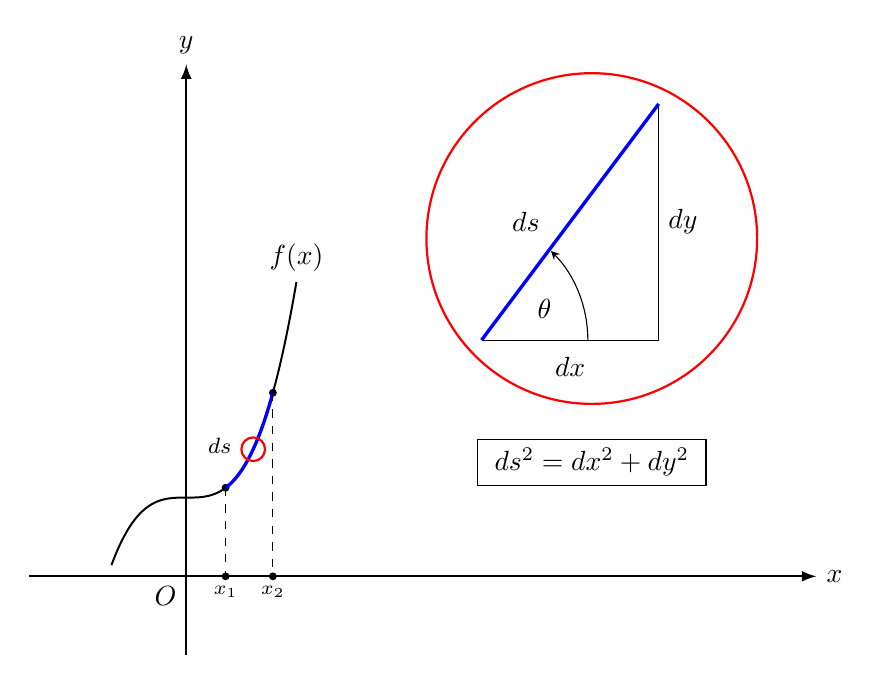
\begin{tikzpicture} [every edge quotes/.append style = {anchor=south, sloped},declare function={f(\x)=1 + \x*\x*\x;}]		% define f(x)
       \draw[thick, -latex] (-2,0) -- (8.0,0.0) coordinate [label={[right] $x$}];  											% x axis
       \draw[thick, -latex] (0,-1) -- (0,6.5) coordinate [label={[above] $y$}]; 											% y axis
       \draw [line width=0.25mm, smooth,samples=100,domain=-0.95:1.40] plot (\x,{f(\x)});									% draw f(x)
       \draw [draw=none] (1.40, {f(1.40)}) coordinate [label={[above] $f(x)$}];												% label f(x)
       \coordinate (O) at (0,0); 																							% origin
       \path (O) node[below left] {$O$};																					% draw origin
%
%	various coordinates
%     
       \coordinate (x1y1) at (0.5,{f(0.5)});
       \coordinate (x1y0) at (0.5,0.0);
       \coordinate (x2y2) at (1.1,{f(1.1});
       \coordinate (x2y0) at (1.1,0.0);
       \coordinate (cir)  at (0.85,{f(0.85)});
%
       \fill (x1y1) circle (0.05);																					% put a dot on the curve at x1y1
       \fill (x2y2) circle (0.05);																					% put a dot on the curve at x2y2
	   \draw [very thick,blue,smooth,samples=100,domain=0.5:1.1] plot (\x,{f(\x)});									% draw blue segment on f(x)
       \draw[draw=none] (x1y1) -- (x2y2) coordinate [label={[font=\footnotesize,yshift=-0.065cm,xshift=-0.105cm,midway,left] \color{black} $ds$}];
       \draw[dashed] (x1y1) -- (x1y0) coordinate [label={[font=\scriptsize,below] \color{black} $x_1$}];
       \draw[dashed] (x2y2) -- (x2y0) coordinate [label={[font=\scriptsize,below] \color{black} $x_2$}];
       \fill (x1y0) circle (0.05);																					% put a dot on the x axis at x1
       \fill (x2y0) circle (0.05);																					% put a dot on the x axis at x2
       \draw[red, thick] (cir) circle (0.150);																		% put a circle on f(x) where ds is
%
%	draw triangle and circle to show ds
%   
%
%
%	set up triangle coordinates
%
	   \coordinate (a) at (3.75,3.00);
	   \coordinate (c) at (6.00,3.00);
	   \coordinate (b) at (6.00,6.00);
%
%	draw the triangle
%	   
       \draw[] (a) -- (c) coordinate [label={[yshift=-0.1cm,midway,below] ${dx}$}];										% dx
       \draw[] (c) -- (b) coordinate [label={[midway,right] ${dy}$}];													% dy
       \draw[blue,very thick] (a) -- (b) coordinate [label={[xshift=-0.25cm,midway,left] \color{black} ${ds}$}];		% ds
       \draw[red,thick] (5.15,4.29) circle (2.10);																		% big circle
       \draw[draw=none] (0,0) -- (5.15,1.75)  node[draw,rectangle,below] {${\; ds^2 = dx^2 + dy^2 \;}$};				% draw the pythagorean theorem
%
%	draw the angle      
%       
       \node[xshift=-2mm, yshift=-2mm] at (4.75,3.60) {$\theta$};
       \draw[-stealth,thin] (5.10,3.00) arc (0:45:1.60cm);
%
%	done
%
     \end{tikzpicture}
    }																					 								% end resizebox                                                            
 \caption{$f(x)$, $ds$ and the Pythagorean Theorem}
 \label{fig:pythagorean_theorem}
\end{figure}


% \begin{figure}[H]
%  \centering
% \resizebox{0.30 \textwidth}{!} {																				% resize the figure if you want
%    \begin{tikzpicture}[framed]
%      \draw [red] (0,0) coordinate[] (a) --
%            	   (3,0) coordinate[] (c) --
%            	   (3,3) coordinate[] (b) -- cycle;
%       \draw[draw=none] (a) -- (c) coordinate [label={[yshift=-0.1cm,midway,below]					${dx}$}];    % dx
%       \draw[draw=none] (c) -- (b) coordinate [label={[xshift=0.025,midway,right]  				${dy}$}];    % dy
%       \draw[draw=none] (a) -- (b) coordinate [label={[xshift=-0.2cm,yshift=0.025cm,midway,left]	${ds}$}];    % ds
%    \end{tikzpicture}
%  }
% \caption{$ds^2 = dx^2 + dy^2$}
% \label{fig:pythagorean_theorem}
%\end{figure}



\bigskip
\bigskip
\bigskip


\begin{figure}[H]
\centering
  \resizebox{0.55 \textwidth}{!} {	

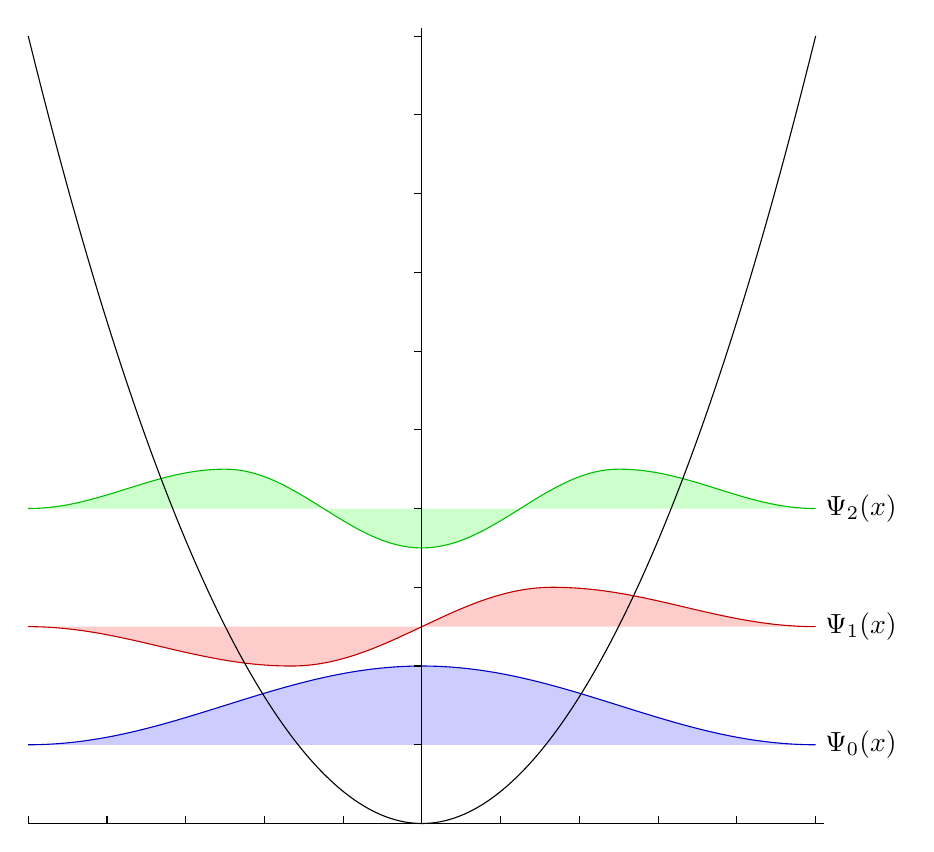
\begin{tikzpicture}
    \def\lzero{(-5,1) cos (-2.5,1.5) sin (0,2) cos (2.5,1.5) sin (5,1)};
  \fill[blue,opacity=0.2] \lzero;
  \draw[blue!75!black] \lzero node[right,black] {$\Psi_0(x)$};

  \def\lone{(-5,2.5) cos (-3.33,2.25) sin (-1.66,2) cos (0,2.5) sin (1.66,3) cos (3.33,2.75) sin (5,2.5)}
  \fill[red,opacity=0.2] \lone;
  \draw[red!75!black] \lone node[right,black] {$\Psi_1(x)$};

  \def\ltwo{(-5,4) cos (-3.75,4.25) sin (-2.5,4.5) cos (-1.25,4) sin (0,3.5) cos (1.25,4) sin (2.5,4.5) cos (3.75,4.25) sin (5,4)}
  \fill[green,opacity=0.2] \ltwo;
  \draw[green!75!black] \ltwo node[right,black] {$\Psi_2(x)$};

  \draw (0,0) parabola (5,10);
  \draw (0,0) parabola (-5,10);

  \begin{scope}[decoration={border, segment length=1cm, amplitude=1mm, angle=90}]
    \draw[postaction={decorate,draw}] (-5,0) -- (5.1,0);
    \draw[postaction={decorate,draw}] (0,0) -- (0,10.1); 
  \end{scope}
\end{tikzpicture}
  }                                                                   								% end resizebox
  \caption{Wave Functions}
  \label{fig:wave_functions}
\end{figure}


\begin{figure}[H]
\centering
  \resizebox{0.55 \textwidth}{!} {	

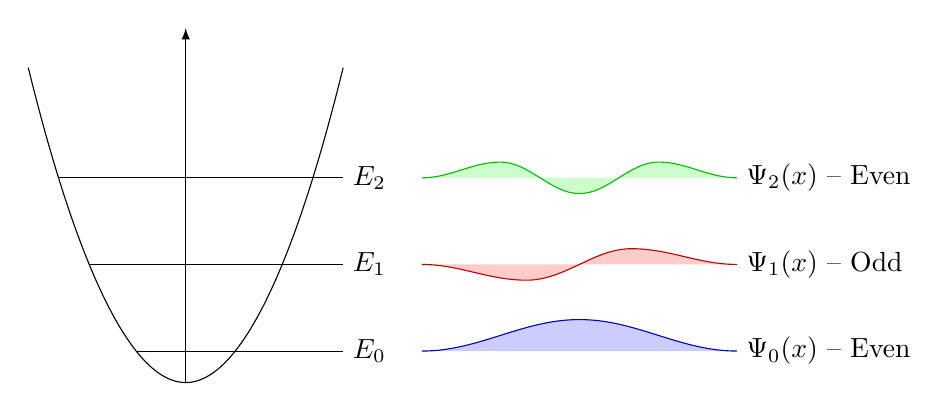
\begin{tikzpicture}
\draw[->] (0,0) -- (0,4.5);

\def\lzero{(3,0.4) cos (4,0.6) sin (5,0.8) cos (6,0.6) sin (7,0.4)};
\fill[blue,opacity=0.2] \lzero;
\draw[blue!75!black] \lzero node[right,black] {$\Psi_0(x)$ \textendash ~Even};
\draw (-0.632,0.4) -- (2,0.4) node[right] {$E_0$};

\def\lone{(3,1.5) cos (3.66,1.4) sin (4.33,1.3) cos (5,1.5) sin (5.66,1.7) cos (6.33,1.6) sin (7,1.5)};
\fill[red,opacity=0.2] \lone;
\draw[red!75!black] \lone node[right,black] {$\Psi_1(x)$ \textendash ~Odd};
\draw (-1.224,1.5) -- (2,1.5) node[right] {$E_1$};

\def\ltwo{(3,2.6) cos (3.5,2.7) sin (4,2.8) cos (4.5,2.6) sin (5,2.4) cos (5.5,2.6) sin (6,2.8) cos (6.5,2.7) sin (7,2.6)};
\fill[green,opacity=0.2] \ltwo;
\draw[green!75!black] \ltwo node[right,black] {$\Psi_2(x)$ \textendash ~Even};
\draw (-1.61,2.6) -- (2,2.6) node[right] {$E_2$};


\draw (0,0) parabola (2,4);
\draw (0,0) parabola (-2,4);
\end{tikzpicture}
  }                                                                   								% end resizebox
  \caption{Wave Functions}
  \label{fig:wave_functions}
\end{figure}



\begin{figure}[H]
 \centering
  \fbox{\begin{minipage}{34em}
    \begin{equation*}
     \begin{array}{rlrlrlr}
       9^2      &=& 81           &\longrightarrow& 8 + 1           &=&  9     \\
       45^2     &=& 2025         &\longrightarrow& 20 + 25         &=& 45     \\
       703^2    &=& 494209       &\longrightarrow& 494 + 209       &=& 703    \\
       7777^2   &=& 60481729     &\longrightarrow& 6048 + 1729     &=& 7777   \\
       857143^2 &=& 734694122449 &\longrightarrow& 734694 + 122449 &=& 857143 \\
     \end{array}
    \end{equation*}
  \end{minipage}}
  \caption{A Few Example Kaprekar Numbers}
\end{figure}

%
%	triangle inequality
%
\begin{figure}[H]
\centering
  \resizebox{0.55 \textwidth}{!} {	
    \tikzstyle{background rectangle}=[thin,draw=black]												% make the frame thinner (there must be an easier way)
    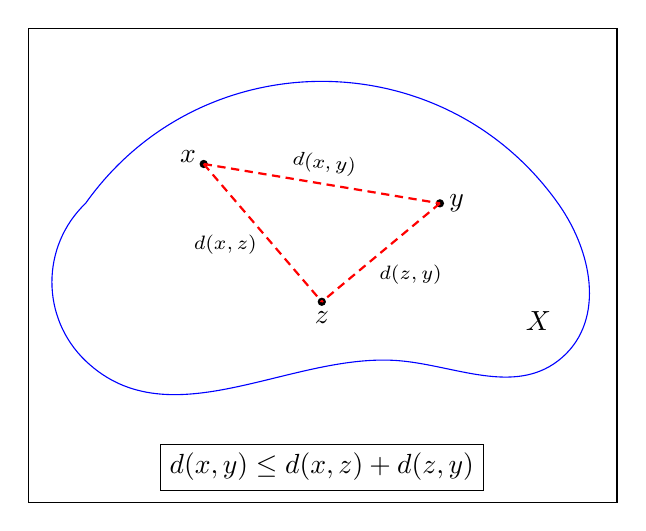
\begin{tikzpicture}[use Hobby shortcut, show background rectangle]								% couldn't control thickness with \begin{tikzpicture} [framed]
%
%	\begin{tikzpicture}[use Hobby shortcut]
%														
%	coordinate system
%
		\coordinate (x)   at (1.50,-5.50);															% x endpoint of dashed line
		\coordinate (xb)  at (1.80,-5.15);															% x endpoint of the brace
		\coordinate (y)   at (4.50,-6.00);															% y endpoint of the dashed line
		\coordinate (yb)  at (4.40,-5.58);															% y endpoint of the brace
		\coordinate (z)   at (3.00,-7.25);															% need a point z for the triangle inequality
		\coordinate (X)   at (5.75,-7.50);															% show X (the whole set) in lower right
		\coordinate (TIL) at (2.25,-8.25);															% left side of triangle inequality
		\coordinate (TIR) at (3.75,-8.25);															% right side of triangle inequality

%
%	draw everything
%
		\draw [draw=blue, rotate=-90, scale=2] 														% draw the (blue) set boundary through these points
		       (3,0) .. +(1,0) .. +(1,2) .. +(1,3) .. +(0,3) .. (3,0);								% make the boundary go through these points
		\fill [fill=black] (x) circle (1.50pt);														% x dot										
		\draw [] (x) node[left, above, , xshift=-2.00mm, yshift=-1.00mm]{$x$}; 						% label x
		\fill [fill=black] (y) circle (1.50pt);														% y dot												
		\draw [] (y) node[right, xshift=-0.05mm]{$y$}; 												% label y
		\fill [fill=black] (z) circle (1.50pt);														% z dot
		\draw [] (z) node[below, yshift=-0.05mm]{$z$}; 												% label z
		\draw [densely dashed, thick, draw=red] (x) -- (y) 											% draw x -- y
		       node[font=\scriptsize, rotate=-7.00, above, midway] {$d(x,y)$};	   					% draw d(x,y)
		\draw [densely dashed, thick, draw=red] (x) -- (z) 											% draw x -- z
		       node[font=\scriptsize, xshift=-4.75mm, yshift=1.00mm, below, midway] {$d(x,z)$};		% draw d(x,z)
		\draw [densely dashed, thick, draw=red] (y) -- (z) 											% draw z -- y
		       node[font=\scriptsize, xshift=-1.50mm, yshift=-2.75mm, right, midway] {$d(z,y)$}; 	% draw d(z,y)
		\draw  [draw=none] (TIL) -- (TIR) 															% draw the definition of the triangle inequality
				node[rectangle, draw, very thin, below, midway, yshift=-0.80cm]						% ...
				{$d(x,y) \leq d(x,z) + d(z,y)$};													% definition of the triangle inequality
		\node [] at (X) {$X$};																		% draw X in the lower right corner
  \end{tikzpicture} 																				% end tikzpicture
  }                                                                   								% end resizebox
  \caption{The Triangle Inequality}
  \label{fig:triangle_inequality}
\end{figure}



\begin{figure}[H]
\centering
  \resizebox{0.53 \textwidth}{!} {	
    \tikzstyle{background rectangle}=[thin,draw=black]												% make the frame thinner (there must be an easier way)
    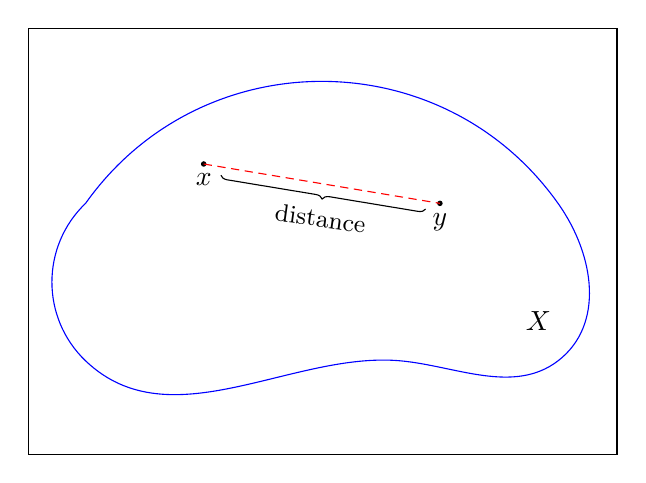
\begin{tikzpicture}[use Hobby shortcut, show background rectangle]								% couldn't control thickness with \begin{tikzpicture} [framed]
%
%	\begin{tikzpicture}[use Hobby shortcut]
%														
%	coordinate system
%
		\coordinate (x)  at (1.50,-5.50);															% x endpoint of dashed line
		\coordinate (xb) at (1.80,-5.15);															% x endpoint of the brace
		\coordinate (y)  at (4.50,-6.00);															% y endpoint of the dashed line
		\coordinate (yb) at (4.40,-5.58);															% y endpoint of the brace					
		\coordinate (X)  at (5.75,-7.50);															% show X (the whole set) in lower right
%
%	draw everything
%
		\draw [draw=blue, rotate=-90, scale=2] 														% draw the (blue) set boundary through these points
		       (3,0) .. +(1,0) .. +(1,2) .. +(1,3) .. +(0,3) .. (3,0);								% make the boundary go through these points
		\fill [fill=black] (x) circle (1pt);														% x dot										
		\draw [] (x) node[below]{$x$}; 																% label x
		\fill [fill=black] (y) circle (1pt);														% y dot												
		\draw [] (y) node[below]{$y$}; 																% label y
		\draw [densely dashed, draw=red] (x) -- (y);    											% draw the dashed line between x and y
		\draw [decoration={brace,mirror,raise=0.5cm},decorate] (xb) -- (yb) 						% draw the underbrace
			node [rotate=-8.00,pos=0.5,anchor=north,yshift=-0.60cm] {${\small \text{distance}}$};	% label it with "distance"	
		\node [] at (X) {$X$};																		% draw X in the lower right corner
  \end{tikzpicture} 																				% end tikzpicture
  }                                                                   								% end resizebox
  \caption{$X,x \text{ and } y$}
  \label{fig:set}
\end{figure}




%
%	open epsilon ball
%
\begin{figure}[H]
\centering
  \resizebox{0.60 \textwidth}{!} {														% resize the tikzpicture if you like
  \tikzstyle{background rectangle}=[thin,draw=black]									% make the frame thinner (there must be an easier way to do this)
     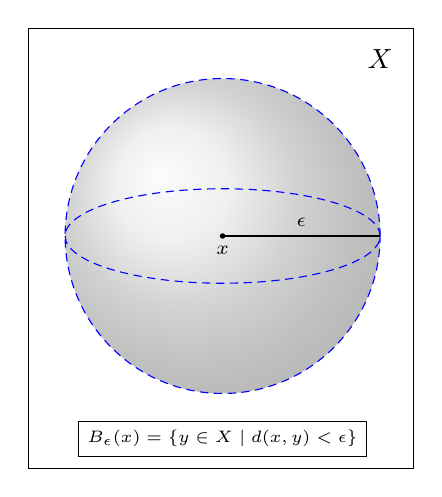
\begin{tikzpicture}[show background rectangle]										% couldn't control frame thickness with \begin{tikzpicture} [framed]
       \coordinate (C)  at (0.00, 0.00);												% center
       \coordinate (R)  at (2.00, 0.00);												% radius
       \coordinate (A)  at (-2.00,0.00);												% arc (3D effect)
       \coordinate (RC) at (2.00, 2.25);												% Right Corner (RC)
       \coordinate (S)  at (-2.20,2.25);												% Spacing
       \shade [ball color = gray!40, opacity = 0.4] (0,0) circle (2cm);					% draw the ball
       \draw  [densely dashed, draw=blue] (C) circle (2cm);								% draw the circle (use dashed because its an open ball)
       \draw  [densely dashed, draw=blue] (A) arc (180:360:2 and 0.6);					% 3D effect
       \draw  [densely dashed, draw=blue] (R) arc (0:180:2 and 0.6);					% draw the dashed line
       \fill  [fill=black] (C) circle (1pt);											% draw a dot in the center
       \draw  [draw=none]  (C) node[font=\scriptsize, below] {$x$};        				% label x
       \draw  [thin] (C) -- (R) node[font=\scriptsize,midway,above]{$\epsilon$};		% draw the radius (epsilon)
       \node  [] at  (RC) {$X$};														% show X in the lower right corner
       \draw  [draw=none] (-2,-1.5) -- (2,-1.5) 										% draw the definition of the epsilon ball
				node[font=\fontsize{6.0}{1.0}\selectfont,rectangle, draw, very thin, below, midway, yshift=-0.85cm] 
				{$B_{\epsilon}(x) =\{y \in X \mid d(x,y) < \epsilon\}$};				% defn of open epsilon ball
       \node  [] at (S) {};																% stretch out the frame so the ball is centered (Spacing)
     \end{tikzpicture}																	% end tikzpicture
    }                                                                   				% end resizebox
    \caption{$B_{\epsilon}(x)$ is an open epsilon ball centered at $x$ with radius $\epsilon$}
    \label{fig:open_epsilon_ball}
\end{figure}



%
% bloch sphere
%
\bigskip
\begin{figure}[H]
\centering
  \resizebox{0.70 \textwidth}{!} {	
  
  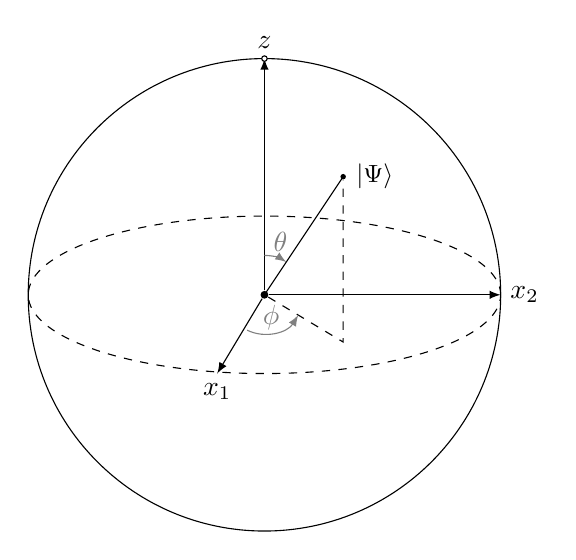
\begin{tikzpicture}

  % Define radius
  \def\r{3}

  % Bloch vector
  \draw (0, 0) node[circle, fill, inner sep=1] (orig) {} -- (\r/3, \r/2) node[circle, fill, inner sep=0.7, label=right:{\small ${\ket{\Psi}}$}] (a) {};
  \draw[dashed] (orig) -- (\r/3, -\r/5) node (phi) {} -- (a);

  % Sphere
  \draw (orig) circle (\r);
  \draw[dashed] (orig) ellipse (\r{} and \r/3);

  % Axes
  \draw[->] (orig) -- ++(-\r/5, -\r/3) node[below] (x1) {$x_1$};
  \draw[->] (orig) -- ++(\r, 0) node[right] (x2) {$x_2$};
  \draw[->] (orig) -- ++(0, \r) node[above] (x3) {$z$};
  \draw[fill=white] (0,\r) circle (0.035);   									% draw center of circle




  % Angles
  \pic [draw=gray, text=gray, ->, "$\phi$"] {angle = x1--orig--phi};
  \pic [draw=gray, text=gray, <-, "$\theta$", angle eccentricity=1.4] {angle = a--orig--x3};

\end{tikzpicture}
     
  }																					 								% end resizebox                                                            
 \caption{The Bloch Sphere}
 \label{fig:bloch_sphere}
\end{figure}
																						% resize figure if you want



%
%	draw Pythagorean theorem stuff
%
\bigskip
\begin{figure}[H]
\centering
  \resizebox{0.70 \textwidth}{!} {																							% resize figure if you want
  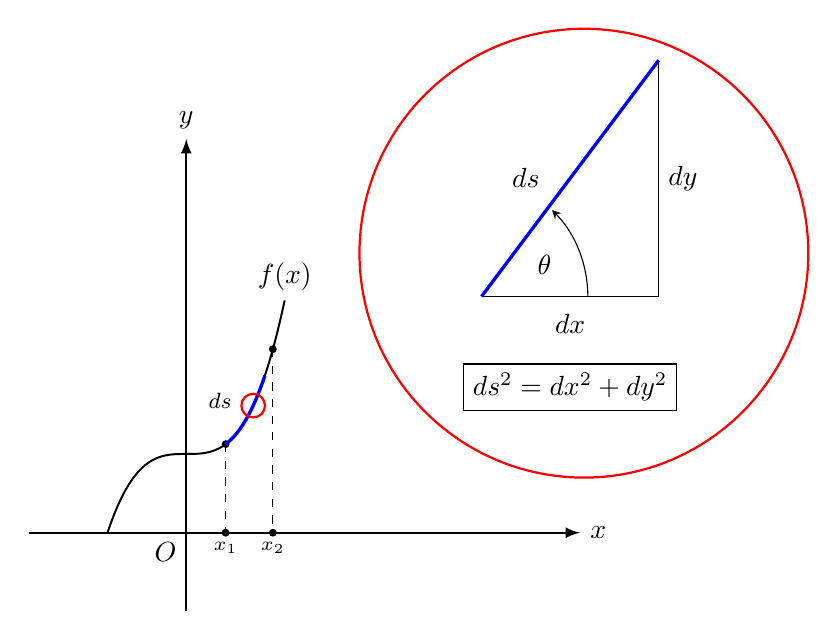
\begin{tikzpicture} [every edge quotes/.append style = {anchor=south, sloped}, declare function={f(\x)=1 + \x*\x*\x;}]	% define f(x)
       \draw[thick, -latex] (-2,0) -- (5,0) coordinate [label={[right] $x$}];  												% x axis
       \draw[thick, -latex] (0,-1) -- (0,5) coordinate [label={[above] $y$}]; 												% y axis
       \draw [line width=0.25mm, smooth, samples=100,domain=-1.0:1.25] plot (\x,{f(\x)});									% draw f(x)
       \draw [draw=none] (1.25, {f(1.25)}) coordinate [label={[above] $f(x)$}];												% label f(x)
       \coordinate (O) at (0,0); 
       \path (O) node[below left] {$O$};  
%
%	various coordinates
%     
       \coordinate (x1y1) at (0.5,{f(0.5)});
       \coordinate (x1y0) at (0.5,0.0);
       \coordinate (x2y2) at (1.1,{f(1.1});
       \coordinate (x2y0) at (1.1,0.0);
       \coordinate (cir) at (0.85,{f(0.85)});
%
       \fill (x1y1) circle (0.05);																					% put a dot on the curve at x1y1
       \fill (x2y2) circle (0.05);																					% put a dot on the curve at x2y2
	   \draw [very thick,blue,smooth,samples=100,domain=0.5:1.0] plot (\x,{f(\x)});									% draw blue segment on f(x)
       \draw[draw=none] (x1y1) -- (x2y2) coordinate [label={[font=\footnotesize, yshift=-0.05cm, xshift=-0.10cm, midway,left] \color{black} $ds$}];
       \draw[dashed] (x1y1) -- (x1y0) coordinate [label={[font=\scriptsize,below] \color{black} $x_1$}];
       \draw[dashed] (x2y2) -- (x2y0) coordinate [label={[font=\scriptsize,below] \color{black} $x_2$}];
       \fill (x1y0) circle (0.05);																					% put a dot on the x axis at x1
       \fill (x2y0) circle (0.05);																					% put a dot on the x axis at x2
       \draw[red, thick] (cir) circle (0.150);																		% put a circle on f(x) where ds is
       

     
%
%	draw triangle and circle to show ds
%   
%
%
%	set up triangle coordinates
%
	   \coordinate (a) at (3.75,3.00);
	   \coordinate (c) at (6.00,3.00);
	   \coordinate (b) at (6.00,6.00);
%
%	draw the triangle
%	   
       \draw[] (a) -- (c) coordinate [label={[yshift=-0.1cm,midway,below] ${dx}$}];										% dx
       \draw[] (c) -- (b) coordinate [label={[midway,right] ${dy}$}];													% dy
       \draw[blue,very thick] (a) -- (b) coordinate [label={[xshift=-0.25cm,midway,left] \color{black} ${ds}$}];		% ds
       \draw[draw=none]  (a) -- (c) node[draw,rectangle,yshift=-0.85cm,midway,below] {${ds^2 = dx^2 + dy^2}$};			% draw the pythagorean theorem
       \draw[red,thick] (5.05,3.55) circle (2.85);																		% big circle
%
%	draw the angle      
%       
       \node[xshift=-2mm, yshift=-2mm] at (4.75,3.60) {$\theta$};
       \draw[-stealth,thin] (5.10,3.00) arc (0:45:1.55cm);
%
%	done
%
     \end{tikzpicture}
    }																					 								% end resizebox                                                            
 \caption{$f(x)$, $ds$ and the Pythagorean Theorem}
 \label{fig:pythagorean_theorem}
\end{figure}



%
% old
%
%
%	draw Pythagorean theorem stuff
%
\bigskip
\begin{figure}[H]
\centering
  \resizebox{0.70 \textwidth}{!} {																							% resize figure if you want
  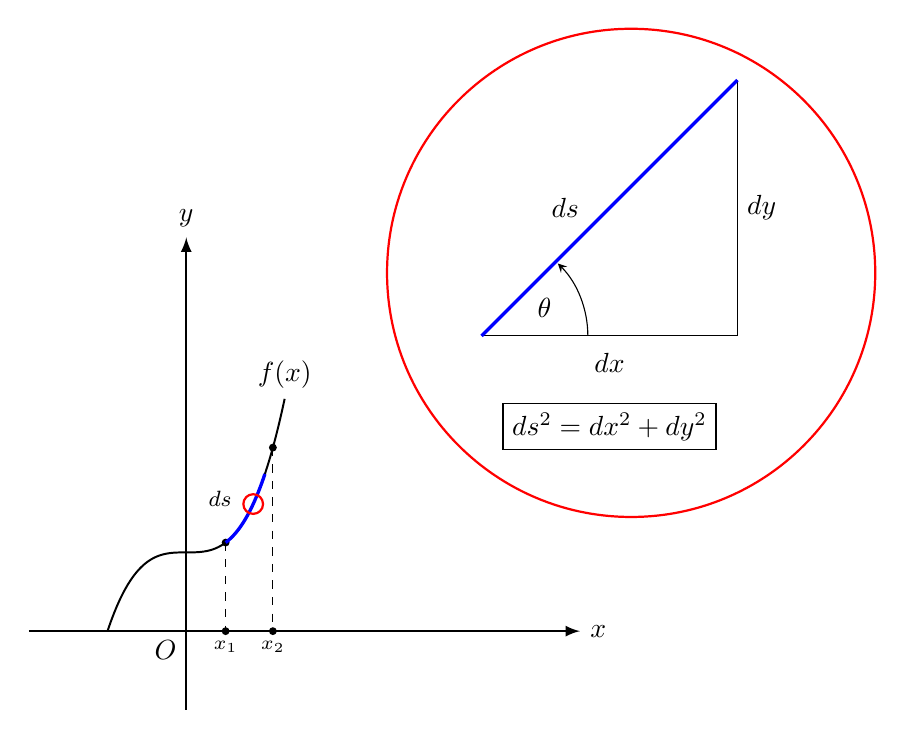
\begin{tikzpicture} [every edge quotes/.append style = {anchor=south, sloped}, declare function={f(\x)=1 + \x*\x*\x;}]	% define f(x)
       \draw[thick, -latex] (-2,0) -- (5,0) coordinate [label={[right] $x$}];  												% x axis
       \draw[thick, -latex] (0,-1) -- (0,5) coordinate [label={[above] $y$}]; 												% y axis
       \draw [line width=0.25mm, smooth, samples=100,domain=-1.0:1.25] plot (\x,{f(\x)});									% draw f(x)
       \draw [draw=none] (1.25, {f(1.25)}) coordinate [label={[above] $f(x)$}];												% label f(x)
       \coordinate (O) at (0,0); 
       \path (O) node[below left] {$O$};  
%
%	various coordinates
%     
       \coordinate (x1y1) at (0.5,{f(0.5)});
       \coordinate (x1y0) at (0.5,0.0);
       \coordinate (x2y2) at (1.1,{f(1.1});
       \coordinate (x2y0) at (1.1,0.0);
       \coordinate (cir) at (0.85,{f(0.85)});
%
       \fill (x1y1) circle (0.05);																					% put a dot on the curve at x1y1
       \fill (x2y2) circle (0.05);																					% put a dot on the curve at x2y2
	   \draw [very thick,blue,smooth,samples=100,domain=0.5:1.0] plot (\x,{f(\x)});									% draw blue segment on f(x)
       \draw[draw=none] (x1y1) -- (x2y2) coordinate [label={[font=\footnotesize, yshift=-0.05cm, xshift=-0.10cm, midway,left] \color{black} $ds$}];
       \draw[dashed] (x1y1) -- (x1y0) coordinate [label={[font=\scriptsize,below] \color{black} $x_1$}];
       \draw[dashed] (x2y2) -- (x2y0) coordinate [label={[font=\scriptsize,below] \color{black} $x_2$}];
       \fill (x1y0) circle (0.05);																					% put a dot on the x axis at x1
       \fill (x2y0) circle (0.05);																					% put a dot on the x axis at x2
       \draw[red, thick] (cir) circle (0.125);																		% put a circle on f(x) where ds is
     
%
%	draw triangle and circle to show ds
%   
%
%
%	set up triangle coordinates
%
	   \coordinate (a) at (3.75,3.75);
	   \coordinate (c) at (7.00,3.75);
	   \coordinate (b) at (7.00,7.00);
%
%	draw the triangle
%	   
       \draw[] (a) -- (c) coordinate [label={[yshift=-0.1cm,midway,below] ${dx}$}];										% dx
       \draw[] (c) -- (b) coordinate [label={[midway,right] ${dy}$}];													% dy
       \draw[blue,very thick] (a) -- (b) coordinate [label={[xshift=-0.25cm,midway,left] \color{black} ${ds}$}];				% ds
       \draw[draw=none]  (a) -- (c) node[draw,rectangle,yshift=-0.85cm,midway,below] {${ds^2 = dx^2 + dy^2}$};			% draw the pythagorean theorem
       \draw[red,thick] (5.65,4.55) circle (3.10);																		% big circle
%
%	draw the angle      
%       
       \node[xshift=-2mm, yshift=-2mm] at (4.75,4.30) {$\theta$};
       \draw[-stealth,thin] (5.10,3.75) arc (0:45:1.30cm);
%
%	done
%
     \end{tikzpicture}
    }																					 								% end resizebox                                                            
 \caption{$f(x)$, $ds$ and the Pythagorean Theorem}
 \label{fig:pythagorean_theorem}
\end{figure}




\end{document}
